\newpage
\section{Implementierung PWA}
Schritte der Implementierung
\begin{enumerate}
	\item Einrichten der Entwicklungsumgebung
	\item Initialisierung des Projekts
	\item Installation der Pakete
\end{enumerate}

\subsection{Einrichten der Projektumgebung}
Für die Entwicklung der PWA wird die Entwicklungsumgebung Webstorm von JetBrains gewählt, da sie die viele Routineaufgaben selbstständig beziehungsweise mit geringem Aufwand ausführt. 

Wie für die Entwicklung der meisten modernen Webanwendungen ist die Installation der Node.js Laufzeitumgebung notwendig. Mit dem integrierten Paketmanager npm lassen sich Bibliotheken leicht zum Projekt hinzufügen.
Um die Angular Anwendung automatisiert zu erstellen, ist zuerst die Installation des Angular \acf{cli} erforderlich. Mit dem Konsolenbefehl \texttt{npm install -g @angular/cli} wird npm aufgefordert, die neuste Version der Angular CLI global auf dem System zu installieren.


Mit dem Befehl \texttt{ng new todoapp} wird die Angular CLI (in der Konsole als \texttt{ng} abgekürzt) dazu gebracht, ein Angularprojekt inklusive nötiger Dateistrukturen zu erstellen. 
\begin{wrapfigure}{r}{0.6\textwidth}
	\vspace{-10pt}
	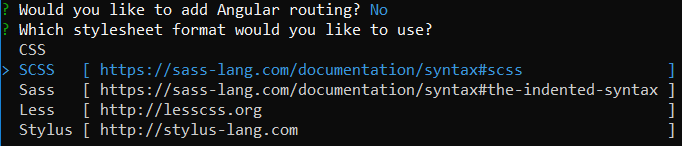
\includegraphics[width=0.58\textwidth]{img/angular_cli_css.PNG}
	\caption{Stylesheetformate beim Erstellen der Angularanwendung}
	\label{fig:stylesheet_formate_cli}
	\vspace{-10pt}
\end{wrapfigure}
Die CLI bietet dem Nutzer einige Optionen bei der Erstellung an, die jedoch in diesem Projekt nicht zwangsläufig benötigt werden, so kann beispielsweise ein Routing oder Unittesting eingerichtet werden.
Außerdem unterstützt die CLI verschiedene Stylesheetformate (siehe Abbildung \ref{fig:stylesheet_formate_cli}). Das ist für Entwickler*innen sehr praktisch, wenn sie einen dieser CSS-Dialekte beherschen. Die Arbeit mit Variablen in Stylesheets bevorzugt wird, werden in diesem Projekt SCSS Dateien verwendet.


\begin{wrapfigure}{r}{0.3\textwidth}
	\vspace{-10pt}
	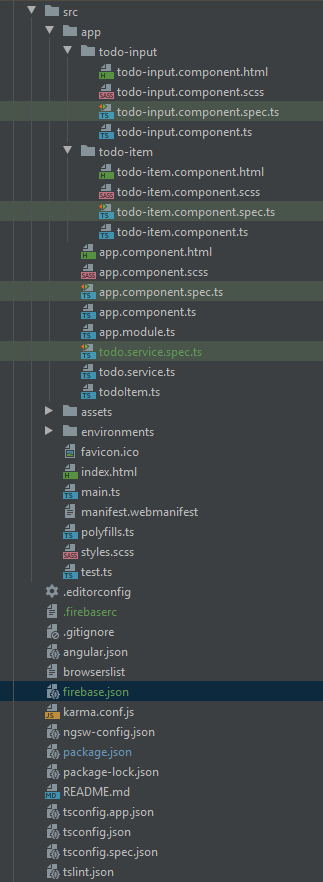
\includegraphics[width=0.28\textwidth]{img/file_tree_pwa.PNG}
	\caption{Dateistruktur des Projekts}
\label{fig:dialog_install_pwa_desktop}
	\vspace{-10pt}
\end{wrapfigure}



\subsection{Angular}
https://www.sitepoint.com/angular-2-tutorial/


\subsection{Hosting der App}
Damit die PWA als solche installiert werden kann muss sie bestimmte Kriterien erfüllen (siehe Kapitel \ref{chap:grundlagen}). Darunter ist die Notwendigkeit der Bereitstellung über HTTPS. Dies gestaltet sich in der Praxis als schwierig, da der Angular Entwicklungsserver zwar auf HTTPS konfiguriert werden kann, jedoch selbstsignierte SSL Zertifikate nicht aktzeptiert werden: Die PWA kann nicht installiert werden. Für die Entwicklung ist das natürlich problematisch, so dass eine Lösung für dieses Problem gefunden werden muss.

Googles stellt eine schnelle und elegante Lösung zum Hosten einer Webanwendung bereit: Firebase. Über die Firebase Console, eine Webanwendung zur Verwaltung von Firebase Projekten, kann innerhalb weniger Minuten ein Projekt inklusive Hosting erstellt werden.

Das dem Firebase CLI können automatisiert Konfigurationsdateien für das Firebase Hosting angelegt werden. Die Schritte dazu sind ebenfalls trivial:
\begin{enumerate}
	\item \textbf{Anmeldung: \\}
	Das CLI muss mit einem Google-Konto verknüpft werden. Dazu beim Login über das CLI ein Browserfenster mit einem Google-Login Dialog.
	\item \textbf{Initialisierung: \\}
	Die Initialisierung über das CLI legt unter anderem eine JSON-Datei zur Konfiguration des Deployments an. Hier werden Dateipfade, wie beispielsweise die Start-URL oder Dateien die deployed werden sollen, gespeichert.
	\item \textbf{Deployment: \\}
	Über die Angular CLI wird ein sogenannter Production-Build erstellt. Dies ist eine gepackte Version der Webanwendung für den Produktivbetrieb.
	Anschließend kann die gepackte Anwendung mit \texttt{firebase deploy} auf einem von Googles Servern bereitgestellt werden.
\end{enumerate}

Die Anwendung läuft jetzt mit einer validen HTTPS-Verbindung und kann von Nutzern installiert werden. 

Das Hosting mit Firebase löst gleichzeitig ein weitere Problem: das Testen der Anwendung auf einem Smartphone. Die von Firebase bereitgestellte URL kann jetzt einfach im mobilen Chromebrowser aufgerufen und installiert werden.

\subsection{Installation der Anwendung}
\textbf{Smartphones:}\\
Nach dem Aufrufen der URL mit dem mobilen Browser, erscheint eine Meldung zum Installieren der PWA (siehe \ref{fig:dialog_install_pwa_mobile}).

\begin{figure}[h]
	
\includegraphics[scale=0.5]{img/pwa_add_to_homescreen.png}
	\centering
	\caption{Browserdialog zum Installieren der PWA als Windows Desktop App}
	\label{fig:dialog_install_pwa_mobile}
\end{figure}

\textbf{Desktop:} 
\begin{wrapfigure}{r}{0.5\textwidth}
		\vspace{-10pt}
	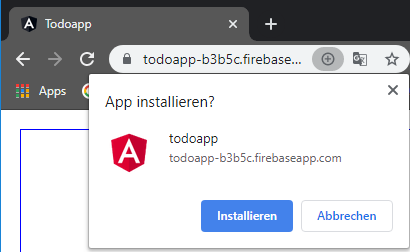
\includegraphics[width=0.48\textwidth]{img/add_to_desktop_2.PNG}
	\caption{Browserdialog zum Installieren der PWA als Desktop App}
	\label{fig:dialog_install_pwa_mobile}
		\vspace{-10pt}
\end{wrapfigure} 
Etwas versteckt in der Suchleiste von Chrome, kann der Nutzer die PWA als Desktopanwendung installieren (siehe \ref{fig:dialog_install_pwa_mobile}).
\begin{wrapfigure}{L}{0.5\textwidth}
		\vspace{-10pt}
	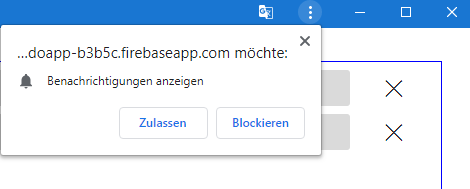
\includegraphics[width=0.48\textwidth]{img/berechtigungen_zulassen.PNG}
	\centering
	\caption{Größen}
	\label{fig:pwa_benachrichtigungen_zulassen}
		\vspace{-10pt}
\end{wrapfigure}
Damit dem Nutzer Benachrichtigungen tatsächlich angezeigt werden, muss er beim erhalten der ersten Nachricht die Benachrichtigungen über einen Dialog aktivieren.

\subsection{Update der Anwendung}


Der Todoanwendung 

Nach einigen Registrierungsschritten wird in der Firebase Console ()ein Projekt 



\subsection{Hinzufügen der Manifestdatei}
https://medium.com/poka-techblog/turn-your-angular-app-into-a-pwa-in-4-easy-steps-543510a9b626

\subsection{Desktop}


Der verwendete Entwicklungsbrowser Chromium bietet keine Möglichkeit die PWA als Desktopanwendung zu installieren.



